\documentclass[]{article}
\usepackage{lmodern}
\usepackage{amssymb,amsmath}
\usepackage{ifxetex,ifluatex}
\usepackage{fixltx2e} % provides \textsubscript
\ifnum 0\ifxetex 1\fi\ifluatex 1\fi=0 % if pdftex
  \usepackage[T1]{fontenc}
  \usepackage[utf8]{inputenc}
\else % if luatex or xelatex
  \ifxetex
    \usepackage{mathspec}
  \else
    \usepackage{fontspec}
  \fi
  \defaultfontfeatures{Ligatures=TeX,Scale=MatchLowercase}
\fi
% use upquote if available, for straight quotes in verbatim environments
\IfFileExists{upquote.sty}{\usepackage{upquote}}{}
% use microtype if available
\IfFileExists{microtype.sty}{%
\usepackage{microtype}
\UseMicrotypeSet[protrusion]{basicmath} % disable protrusion for tt fonts
}{}
\usepackage[margin=1in]{geometry}
\usepackage{hyperref}
\hypersetup{unicode=true,
            pdftitle={CS636 R Assignment 2},
            pdfauthor={Maggie Zhang},
            pdfborder={0 0 0},
            breaklinks=true}
\urlstyle{same}  % don't use monospace font for urls
\usepackage{color}
\usepackage{fancyvrb}
\newcommand{\VerbBar}{|}
\newcommand{\VERB}{\Verb[commandchars=\\\{\}]}
\DefineVerbatimEnvironment{Highlighting}{Verbatim}{commandchars=\\\{\}}
% Add ',fontsize=\small' for more characters per line
\usepackage{framed}
\definecolor{shadecolor}{RGB}{248,248,248}
\newenvironment{Shaded}{\begin{snugshade}}{\end{snugshade}}
\newcommand{\KeywordTok}[1]{\textcolor[rgb]{0.13,0.29,0.53}{\textbf{#1}}}
\newcommand{\DataTypeTok}[1]{\textcolor[rgb]{0.13,0.29,0.53}{#1}}
\newcommand{\DecValTok}[1]{\textcolor[rgb]{0.00,0.00,0.81}{#1}}
\newcommand{\BaseNTok}[1]{\textcolor[rgb]{0.00,0.00,0.81}{#1}}
\newcommand{\FloatTok}[1]{\textcolor[rgb]{0.00,0.00,0.81}{#1}}
\newcommand{\ConstantTok}[1]{\textcolor[rgb]{0.00,0.00,0.00}{#1}}
\newcommand{\CharTok}[1]{\textcolor[rgb]{0.31,0.60,0.02}{#1}}
\newcommand{\SpecialCharTok}[1]{\textcolor[rgb]{0.00,0.00,0.00}{#1}}
\newcommand{\StringTok}[1]{\textcolor[rgb]{0.31,0.60,0.02}{#1}}
\newcommand{\VerbatimStringTok}[1]{\textcolor[rgb]{0.31,0.60,0.02}{#1}}
\newcommand{\SpecialStringTok}[1]{\textcolor[rgb]{0.31,0.60,0.02}{#1}}
\newcommand{\ImportTok}[1]{#1}
\newcommand{\CommentTok}[1]{\textcolor[rgb]{0.56,0.35,0.01}{\textit{#1}}}
\newcommand{\DocumentationTok}[1]{\textcolor[rgb]{0.56,0.35,0.01}{\textbf{\textit{#1}}}}
\newcommand{\AnnotationTok}[1]{\textcolor[rgb]{0.56,0.35,0.01}{\textbf{\textit{#1}}}}
\newcommand{\CommentVarTok}[1]{\textcolor[rgb]{0.56,0.35,0.01}{\textbf{\textit{#1}}}}
\newcommand{\OtherTok}[1]{\textcolor[rgb]{0.56,0.35,0.01}{#1}}
\newcommand{\FunctionTok}[1]{\textcolor[rgb]{0.00,0.00,0.00}{#1}}
\newcommand{\VariableTok}[1]{\textcolor[rgb]{0.00,0.00,0.00}{#1}}
\newcommand{\ControlFlowTok}[1]{\textcolor[rgb]{0.13,0.29,0.53}{\textbf{#1}}}
\newcommand{\OperatorTok}[1]{\textcolor[rgb]{0.81,0.36,0.00}{\textbf{#1}}}
\newcommand{\BuiltInTok}[1]{#1}
\newcommand{\ExtensionTok}[1]{#1}
\newcommand{\PreprocessorTok}[1]{\textcolor[rgb]{0.56,0.35,0.01}{\textit{#1}}}
\newcommand{\AttributeTok}[1]{\textcolor[rgb]{0.77,0.63,0.00}{#1}}
\newcommand{\RegionMarkerTok}[1]{#1}
\newcommand{\InformationTok}[1]{\textcolor[rgb]{0.56,0.35,0.01}{\textbf{\textit{#1}}}}
\newcommand{\WarningTok}[1]{\textcolor[rgb]{0.56,0.35,0.01}{\textbf{\textit{#1}}}}
\newcommand{\AlertTok}[1]{\textcolor[rgb]{0.94,0.16,0.16}{#1}}
\newcommand{\ErrorTok}[1]{\textcolor[rgb]{0.64,0.00,0.00}{\textbf{#1}}}
\newcommand{\NormalTok}[1]{#1}
\usepackage{graphicx,grffile}
\makeatletter
\def\maxwidth{\ifdim\Gin@nat@width>\linewidth\linewidth\else\Gin@nat@width\fi}
\def\maxheight{\ifdim\Gin@nat@height>\textheight\textheight\else\Gin@nat@height\fi}
\makeatother
% Scale images if necessary, so that they will not overflow the page
% margins by default, and it is still possible to overwrite the defaults
% using explicit options in \includegraphics[width, height, ...]{}
\setkeys{Gin}{width=\maxwidth,height=\maxheight,keepaspectratio}
\IfFileExists{parskip.sty}{%
\usepackage{parskip}
}{% else
\setlength{\parindent}{0pt}
\setlength{\parskip}{6pt plus 2pt minus 1pt}
}
\setlength{\emergencystretch}{3em}  % prevent overfull lines
\providecommand{\tightlist}{%
  \setlength{\itemsep}{0pt}\setlength{\parskip}{0pt}}
\setcounter{secnumdepth}{0}
% Redefines (sub)paragraphs to behave more like sections
\ifx\paragraph\undefined\else
\let\oldparagraph\paragraph
\renewcommand{\paragraph}[1]{\oldparagraph{#1}\mbox{}}
\fi
\ifx\subparagraph\undefined\else
\let\oldsubparagraph\subparagraph
\renewcommand{\subparagraph}[1]{\oldsubparagraph{#1}\mbox{}}
\fi

%%% Use protect on footnotes to avoid problems with footnotes in titles
\let\rmarkdownfootnote\footnote%
\def\footnote{\protect\rmarkdownfootnote}

%%% Change title format to be more compact
\usepackage{titling}

% Create subtitle command for use in maketitle
\newcommand{\subtitle}[1]{
  \posttitle{
    \begin{center}\large#1\end{center}
    }
}

\setlength{\droptitle}{-2em}

  \title{CS636 R Assignment 2}
    \pretitle{\vspace{\droptitle}\centering\huge}
  \posttitle{\par}
    \author{Maggie Zhang}
    \preauthor{\centering\large\emph}
  \postauthor{\par}
      \predate{\centering\large\emph}
  \postdate{\par}
    \date{February 20, 2019}


\begin{document}
\maketitle

\subsection{CS636 Homework 2}\label{cs636-homework-2}

Due on Feb 23 2019 Submit hardcopy in class Submit electronic copy in
moodle

Please submit the code together with the running results of the testing
commands. Please do not use existing R packages and functions like
sort(), order() and so on.

\paragraph{1,Write a function, F(x), which takes x asthe input
parameter.It calculates and prints the value of the following
mathematical
function.}\label{write-a-function-fx-which-takes-x-asthe-input-parameter.it-calculates-and-prints-the-value-of-the-following-mathematical-function.}

\begin{figure}
\centering
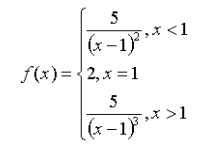
\includegraphics{CS636_R_Assignment_2_Pic.png}
\caption{}
\end{figure}

\paragraph{Testing commands: F(1); F(10);
F(0.3);}\label{testing-commands-f1-f10-f0.3}

\begin{Shaded}
\begin{Highlighting}[]
\NormalTok{F <-}\StringTok{ }\ControlFlowTok{function}\NormalTok{(x) \{}
  
  \CommentTok{# if x < 1 then formula}
  \ControlFlowTok{if}\NormalTok{(x}\OperatorTok{<}\DecValTok{1}\NormalTok{)\{}
  
\NormalTok{    y <-}\StringTok{ }\DecValTok{5}\OperatorTok{/}\NormalTok{((x}\OperatorTok{-}\DecValTok{1}\NormalTok{)}\OperatorTok{^}\DecValTok{2}\NormalTok{)}
  
\NormalTok{  \}}\ControlFlowTok{else} \ControlFlowTok{if}\NormalTok{(x}\OperatorTok{==}\DecValTok{1}\NormalTok{)\{ }\CommentTok{# if x == 1 then 2}
    
\NormalTok{    y <-}\StringTok{ }\DecValTok{2}
  
\NormalTok{  \}}\ControlFlowTok{else} \ControlFlowTok{if}\NormalTok{(x}\OperatorTok{>}\DecValTok{1}\NormalTok{)\{ }\CommentTok{# if x > 1 then formula}
  
\NormalTok{    y <-}\DecValTok{5}\OperatorTok{/}\NormalTok{((x}\OperatorTok{-}\DecValTok{1}\NormalTok{)}\OperatorTok{^}\DecValTok{3}\NormalTok{)}
  
\NormalTok{  \}}
  
  \KeywordTok{return}\NormalTok{(y)}
\NormalTok{\}}

\KeywordTok{F}\NormalTok{(}\DecValTok{1}\NormalTok{)}
\end{Highlighting}
\end{Shaded}

\begin{verbatim}
## [1] 2
\end{verbatim}

\begin{Shaded}
\begin{Highlighting}[]
\KeywordTok{F}\NormalTok{(}\DecValTok{10}\NormalTok{)}
\end{Highlighting}
\end{Shaded}

\begin{verbatim}
## [1] 0.006858711
\end{verbatim}

\begin{Shaded}
\begin{Highlighting}[]
\KeywordTok{F}\NormalTok{(}\FloatTok{0.3}\NormalTok{)}
\end{Highlighting}
\end{Shaded}

\begin{verbatim}
## [1] 10.20408
\end{verbatim}

\paragraph{2, The Fibonacci sequence 1, 1, 2, 3, 5, 8, 13,
21\ldots{}\ldots{} starts with two 1s, and each term afterwards is the
sum of its two predecessors. Please write a function, Fib(n), which
takes n as the input parameter. It will return the n-th number in the
Fibonacci
sequence.}\label{the-fibonacci-sequence-1-1-2-3-5-8-13-21-starts-with-two-1s-and-each-term-afterwards-is-the-sum-of-its-two-predecessors.-please-write-a-function-fibn-which-takes-n-as-the-input-parameter.-it-will-return-the-n-th-number-in-the-fibonacci-sequence.}

\paragraph{Testing commands: Fib(1); Fib(2);
Fib(100);}\label{testing-commands-fib1-fib2-fib100}

\begin{Shaded}
\begin{Highlighting}[]
\CommentTok{# Using List mehtod to calculate}
\NormalTok{Fib <-}\StringTok{ }\ControlFlowTok{function}\NormalTok{(n)\{}
  
\NormalTok{  fiblist <-}\StringTok{ }\KeywordTok{c}\NormalTok{()}
  
  \ControlFlowTok{if}\NormalTok{ (n}\OperatorTok{==}\DecValTok{1}\NormalTok{)\{}
    
\NormalTok{    fiblist[}\DecValTok{1}\NormalTok{] <-}\StringTok{ }\DecValTok{1}
    
\NormalTok{  \}}\ControlFlowTok{else} \ControlFlowTok{if}\NormalTok{(n}\OperatorTok{==}\DecValTok{2}\NormalTok{)\{}
    
\NormalTok{    fiblist[}\DecValTok{1}\NormalTok{] <-}\StringTok{ }\DecValTok{1}
\NormalTok{    fiblist[}\DecValTok{2}\NormalTok{] <-}\StringTok{ }\DecValTok{1}
    
\NormalTok{  \}}\ControlFlowTok{else}\NormalTok{\{}
  
\NormalTok{    fiblist[}\DecValTok{1}\NormalTok{] <-}\StringTok{ }\DecValTok{1}
\NormalTok{    fiblist[}\DecValTok{2}\NormalTok{] <-}\StringTok{ }\DecValTok{1}
    
    \ControlFlowTok{for}\NormalTok{ (i }\ControlFlowTok{in} \DecValTok{3}\OperatorTok{:}\NormalTok{n)\{}

\NormalTok{      fiblist[i] <-}\StringTok{ }\NormalTok{fiblist[i}\OperatorTok{-}\DecValTok{2}\NormalTok{]}\OperatorTok{+}\NormalTok{fiblist[i}\OperatorTok{-}\DecValTok{1}\NormalTok{]}

\NormalTok{    \}}
\NormalTok{  \}}

  \CommentTok{# Turn Scientific Notation Off}
  \KeywordTok{return}\NormalTok{(}\KeywordTok{format}\NormalTok{(fiblist[n],}\DataTypeTok{scientific =} \OtherTok{FALSE}\NormalTok{))}
  
\NormalTok{\}}

\KeywordTok{Fib}\NormalTok{(}\DecValTok{1}\NormalTok{)}
\end{Highlighting}
\end{Shaded}

\begin{verbatim}
## [1] "1"
\end{verbatim}

\begin{Shaded}
\begin{Highlighting}[]
\KeywordTok{Fib}\NormalTok{(}\DecValTok{2}\NormalTok{)}
\end{Highlighting}
\end{Shaded}

\begin{verbatim}
## [1] "1"
\end{verbatim}

\begin{Shaded}
\begin{Highlighting}[]
\KeywordTok{Fib}\NormalTok{(}\DecValTok{100}\NormalTok{)}
\end{Highlighting}
\end{Shaded}

\begin{verbatim}
## [1] "354224848179261997066"
\end{verbatim}

\begin{Shaded}
\begin{Highlighting}[]
\CommentTok{# Using recursive methods to calculate the same.}
\CommentTok{# Using memoise library to improve CPU efficiency}
\KeywordTok{library}\NormalTok{(memoise)}
\NormalTok{Fib <-}\StringTok{ }\KeywordTok{memoise}\NormalTok{(}\ControlFlowTok{function}\NormalTok{(n)\{}
  
  
  
  \ControlFlowTok{if}\NormalTok{ (n}\OperatorTok{==}\DecValTok{1}\NormalTok{)\{}
    
    \KeywordTok{return}\NormalTok{(}\DecValTok{1}\NormalTok{)}
    
\NormalTok{  \}}\ControlFlowTok{else} \ControlFlowTok{if}\NormalTok{(n}\OperatorTok{==}\DecValTok{2}\NormalTok{)\{}
    
    \KeywordTok{return}\NormalTok{(}\DecValTok{1}\NormalTok{)}
    
\NormalTok{  \}}\ControlFlowTok{else}\NormalTok{\{}
  
    \KeywordTok{return}\NormalTok{(}\KeywordTok{Fib}\NormalTok{(n}\OperatorTok{-}\DecValTok{1}\NormalTok{)}\OperatorTok{+}\KeywordTok{Fib}\NormalTok{(n}\OperatorTok{-}\DecValTok{2}\NormalTok{))}

\NormalTok{  \}}

  
\NormalTok{\})}

\KeywordTok{Fib}\NormalTok{(}\DecValTok{1}\NormalTok{)}
\end{Highlighting}
\end{Shaded}

\begin{verbatim}
## [1] 1
\end{verbatim}

\begin{Shaded}
\begin{Highlighting}[]
\KeywordTok{Fib}\NormalTok{(}\DecValTok{2}\NormalTok{)}
\end{Highlighting}
\end{Shaded}

\begin{verbatim}
## [1] 1
\end{verbatim}

\begin{Shaded}
\begin{Highlighting}[]
\KeywordTok{Fib}\NormalTok{(}\DecValTok{100}\NormalTok{)}
\end{Highlighting}
\end{Shaded}

\begin{verbatim}
## [1] 3.542248e+20
\end{verbatim}

\paragraph{3, The merge operation plays an important role in merge sort
algorithm. Suppose you have two sorted sequences S1 and S2, merge
operation will combine these two sequences into a single ordered
sequence. Please write a function, Merge(S1, S2), which accepts two
ordered vectors S1 and S2 as parameters. It will return a single ordered
sequence. For example, S1 = c(1,3,5,7); S2=c(2,4,6,10); Merge(S1, S2)
will return
c(1,2,3,4,5,6,7,10)}\label{the-merge-operation-plays-an-important-role-in-merge-sort-algorithm.-suppose-you-have-two-sorted-sequences-s1-and-s2-merge-operation-will-combine-these-two-sequences-into-a-single-ordered-sequence.-please-write-a-function-merges1-s2-which-accepts-two-ordered-vectors-s1-and-s2-as-parameters.-it-will-return-a-single-ordered-sequence.-for-example-s1-c1357-s2c24610-merges1-s2-will-return-c123456710}

\paragraph{Testing commands: Merge(seq(1, 50, by=3), seq(2, 30,
by=2))}\label{testing-commands-mergeseq1-50-by3-seq2-30-by2}

\begin{Shaded}
\begin{Highlighting}[]
\CommentTok{# Merge Sort}
\NormalTok{Merge <-}\StringTok{ }\ControlFlowTok{function}\NormalTok{ (S1, S2)\{}
  
  \KeywordTok{print}\NormalTok{(}\StringTok{"S1 contains:"}\NormalTok{)}
  \KeywordTok{print}\NormalTok{(S1)}
  \KeywordTok{print}\NormalTok{(}\StringTok{"S2 contains:"}\NormalTok{)}
  \KeywordTok{print}\NormalTok{(S2)}
  
\NormalTok{  len1 <-}\StringTok{ }\KeywordTok{length}\NormalTok{(S1)}
\NormalTok{  len2 <-}\StringTok{ }\KeywordTok{length}\NormalTok{(S2)}
\NormalTok{  len <-}\StringTok{ }\NormalTok{len1 }\OperatorTok{+}\StringTok{ }\NormalTok{len2}
  
\NormalTok{  S <-}\StringTok{ }\KeywordTok{c}\NormalTok{()}
  
\NormalTok{  k1 <-}\StringTok{ }\DecValTok{1}
\NormalTok{  k2 <-}\StringTok{ }\DecValTok{1}
  
  \ControlFlowTok{for}\NormalTok{ (x }\ControlFlowTok{in} \DecValTok{1}\OperatorTok{:}\NormalTok{len)\{}
    
    \ControlFlowTok{if}\NormalTok{(k1}\OperatorTok{>}\NormalTok{len1)\{}
\NormalTok{      S[x}\OperatorTok{:}\NormalTok{len] <-}\StringTok{ }\NormalTok{S2[k2}\OperatorTok{:}\NormalTok{len2]}
      \ControlFlowTok{break}
\NormalTok{    \}}\ControlFlowTok{else} \ControlFlowTok{if}\NormalTok{ (k2}\OperatorTok{>}\NormalTok{len2)\{}
\NormalTok{      S[x}\OperatorTok{:}\NormalTok{len] <-}\StringTok{ }\NormalTok{S1[k1}\OperatorTok{:}\NormalTok{len1] }
      \ControlFlowTok{break}
\NormalTok{    \}}\ControlFlowTok{else} \ControlFlowTok{if}\NormalTok{(S1[k1]}\OperatorTok{<}\NormalTok{S2[k2])\{}
\NormalTok{      S[x] <-}\StringTok{ }\NormalTok{S1[k1]}
\NormalTok{      k1 <-}\StringTok{ }\NormalTok{k1}\OperatorTok{+}\DecValTok{1}
\NormalTok{    \}}\ControlFlowTok{else}\NormalTok{\{}
\NormalTok{      S[x] <-}\StringTok{ }\NormalTok{S2[k2]}
\NormalTok{      k2 <-}\StringTok{ }\NormalTok{k2}\OperatorTok{+}\DecValTok{1}
\NormalTok{    \}}
\NormalTok{  \}}
  
  \KeywordTok{print}\NormalTok{(}\StringTok{"After Merge:"}\NormalTok{)}
  \KeywordTok{return}\NormalTok{(S)}
\NormalTok{\}}

\KeywordTok{Merge}\NormalTok{(}\KeywordTok{seq}\NormalTok{(}\DecValTok{1}\NormalTok{, }\DecValTok{50}\NormalTok{, }\DataTypeTok{by=}\DecValTok{3}\NormalTok{), }\KeywordTok{seq}\NormalTok{(}\DecValTok{2}\NormalTok{, }\DecValTok{30}\NormalTok{, }\DataTypeTok{by=}\DecValTok{2}\NormalTok{))}
\end{Highlighting}
\end{Shaded}

\begin{verbatim}
## [1] "S1 contains:"
##  [1]  1  4  7 10 13 16 19 22 25 28 31 34 37 40 43 46 49
## [1] "S2 contains:"
##  [1]  2  4  6  8 10 12 14 16 18 20 22 24 26 28 30
## [1] "After Merge:"
\end{verbatim}

\begin{verbatim}
##  [1]  1  2  4  4  6  7  8 10 10 12 13 14 16 16 18 19 20 22 22 24 25 26 28
## [24] 28 30 31 34 37 40 43 46 49
\end{verbatim}

\paragraph{4, One of the most important algorithms is the quick sort,
which is based on the quick sort partition. Here we implement a simple
version of the partition function. Please write a function,
Partition(pivot, vect), which takes two parameters. The function
partitions the sequence, vect, into two parts (part1 \textless{}= pivot;
part2 \textgreater{} pivot) based on the pivot. For example, Pivot = 6;
Vect = c(1, 5, 3, 7, 9, 6, 4, 2, 10, 8); List = Partition(Pivot, Vect);
List{[}{[}1{]}{]} is c(1,5,3,4,2, 6) and List{[}{[}2{]}{]} is c(7, 9,
10, 8). Note that Partition returns a
list.}\label{one-of-the-most-important-algorithms-is-the-quick-sort-which-is-based-on-the-quick-sort-partition.-here-we-implement-a-simple-version-of-the-partition-function.-please-write-a-function-partitionpivot-vect-which-takes-two-parameters.-the-function-partitions-the-sequence-vect-into-two-parts-part1-pivot-part2-pivot-based-on-the-pivot.-for-example-pivot-6-vect-c1-5-3-7-9-6-4-2-10-8-list-partitionpivot-vect-list1-is-c15342-6-and-list2-is-c7-9-10-8.-note-that-partition-returns-a-list.}

\paragraph{Testing commands: Partition(50, sample(1:100, 100,
replace=F))}\label{testing-commands-partition50-sample1100-100-replacef}

\begin{Shaded}
\begin{Highlighting}[]
\CommentTok{# Partition list}
\NormalTok{Partition <-}\StringTok{ }\ControlFlowTok{function}\NormalTok{(Pivot, vect)\{}
  
\NormalTok{  len =}\StringTok{ }\KeywordTok{length}\NormalTok{(vect)}
\NormalTok{  list1 <-}\StringTok{ }\KeywordTok{c}\NormalTok{()}
\NormalTok{  list2 <-}\StringTok{ }\KeywordTok{c}\NormalTok{()}
\NormalTok{  k1 <-}\StringTok{ }\DecValTok{1}
\NormalTok{  k2 <-}\StringTok{ }\DecValTok{1}
  
  \ControlFlowTok{for}\NormalTok{(x }\ControlFlowTok{in} \DecValTok{1}\OperatorTok{:}\NormalTok{len)\{}
    \ControlFlowTok{if}\NormalTok{ (vect[x]}\OperatorTok{<=}\NormalTok{Pivot)\{}
\NormalTok{      list1[k1] <-}\StringTok{ }\NormalTok{vect[x]}
\NormalTok{      k1 <-}\StringTok{ }\NormalTok{k1}\OperatorTok{+}\DecValTok{1}
\NormalTok{    \}}\ControlFlowTok{else}\NormalTok{\{}
\NormalTok{      list2[k2] <-}\StringTok{ }\NormalTok{vect[x]}
\NormalTok{      k2 <-}\StringTok{ }\NormalTok{k2}\OperatorTok{+}\DecValTok{1}
\NormalTok{    \}}
    
\NormalTok{  \}}
  
\NormalTok{  listt =}\StringTok{ }\KeywordTok{list}\NormalTok{(list1,list2)}
  
  \KeywordTok{return}\NormalTok{(listt)}
  
\NormalTok{\}}

\KeywordTok{Partition}\NormalTok{(}\DecValTok{50}\NormalTok{, }\KeywordTok{sample}\NormalTok{(}\DecValTok{1}\OperatorTok{:}\DecValTok{100}\NormalTok{, }\DecValTok{100}\NormalTok{, }\DataTypeTok{replace=}\OtherTok{FALSE}\NormalTok{))}
\end{Highlighting}
\end{Shaded}

\begin{verbatim}
## [[1]]
##  [1] 14 16 38 33 13 30 48 11  8 20 28 23 31  7 21 25 40 34  9 24 29 32 35
## [24] 43 26 45 46  5 17  4 22 42 47 15 49 27  2 39 18 50  1 12 10 19 37 36
## [47]  3 44 41  6
## 
## [[2]]
##  [1]  64  53  66  59  61  97  88  60  95  98  73  84  57  83  54  72  51
## [18]  69  86  77  85  68  79  93  80  65  90  67  81  70  76  63  74  52
## [35]  75  91  92  82  62  89  96  71  56  55  94  58  99  87 100  78
\end{verbatim}

\begin{Shaded}
\begin{Highlighting}[]
\CommentTok{# Quick Sort}
\NormalTok{Quick <-}\StringTok{ }\ControlFlowTok{function}\NormalTok{(vect)\{}
  
  
\NormalTok{  vavg <-}\StringTok{ }\KeywordTok{mean}\NormalTok{(vect)}
  
\NormalTok{  list <-}\StringTok{ }\KeywordTok{Partition}\NormalTok{(vavg,vect)}
  
\NormalTok{  len1 =}\StringTok{ }\KeywordTok{length}\NormalTok{(list[[}\DecValTok{1}\NormalTok{]])}
\NormalTok{  len2 =}\StringTok{ }\KeywordTok{length}\NormalTok{(list[[}\DecValTok{2}\NormalTok{]])}

  \ControlFlowTok{if}\NormalTok{(len1}\OperatorTok{>}\DecValTok{1}\NormalTok{)\{}
\NormalTok{    list1 <-}\StringTok{ }\KeywordTok{Quick}\NormalTok{(list[[}\DecValTok{1}\NormalTok{]])}
\NormalTok{  \}}\ControlFlowTok{else}\NormalTok{\{}
\NormalTok{    list1 <-}\StringTok{ }\NormalTok{list[[}\DecValTok{1}\NormalTok{]]}
\NormalTok{  \}}
  
  \ControlFlowTok{if}\NormalTok{(len2}\OperatorTok{>}\DecValTok{1}\NormalTok{)\{}
\NormalTok{    list2 <-}\StringTok{ }\KeywordTok{Quick}\NormalTok{(list[[}\DecValTok{2}\NormalTok{]])}
\NormalTok{  \}}\ControlFlowTok{else}\NormalTok{\{}
\NormalTok{    list2 <-}\StringTok{ }\NormalTok{list[[}\DecValTok{2}\NormalTok{]]}
\NormalTok{  \}}
  
  
\NormalTok{  listt =}\StringTok{ }\KeywordTok{c}\NormalTok{(list1,list2)}
  
  \KeywordTok{return}\NormalTok{(listt)}
\NormalTok{\}}

\KeywordTok{Quick}\NormalTok{(}\KeywordTok{sample}\NormalTok{(}\DecValTok{1}\OperatorTok{:}\DecValTok{100}\NormalTok{, }\DecValTok{100}\NormalTok{, }\DataTypeTok{replace=}\OtherTok{FALSE}\NormalTok{))}
\end{Highlighting}
\end{Shaded}

\begin{verbatim}
##   [1]   1   2   3   4   5   6   7   8   9  10  11  12  13  14  15  16  17
##  [18]  18  19  20  21  22  23  24  25  26  27  28  29  30  31  32  33  34
##  [35]  35  36  37  38  39  40  41  42  43  44  45  46  47  48  49  50  51
##  [52]  52  53  54  55  56  57  58  59  60  61  62  63  64  65  66  67  68
##  [69]  69  70  71  72  73  74  75  76  77  78  79  80  81  82  83  84  85
##  [86]  86  87  88  89  90  91  92  93  94  95  96  97  98  99 100
\end{verbatim}


\end{document}
